\documentclass[11pt, oneside]{article}   	% use "amsart" instead of "article" for
\usepackage{geometry}            	% See geometry.pdf to learn the layout options. 
\geometry{letterpaper, margin=1in}              	% ... or a4paper or a5paper or ... 
\usepackage{graphicx}				% Use pdf, png, jpg, or eps§ with pdflatex; use 	
\usepackage{amssymb}
\usepackage{booktabs}
\usepackage[font=small,labelfont=bf]{caption}
\usepackage{titling}
\usepackage[printwatermark]{xwatermark}
\usepackage{xcolor}
\usepackage{graphicx}
\usepackage{tikz}
\usepackage{lipsum}
\usepackage{multirow}

\setlength{\droptitle}{-8em}

\usepackage{fancyhdr}
\pagestyle{fancy} % enable fancy page style
\fancyfoot[R]{ % right
%    \includegraphics[scale=0.9]{../ARSlogo.png}
}

\newsavebox\mybox
\savebox\mybox{\tikz[color=red,opacity=0.6]\node{DO NOT DISTRIBUTE};}
\newwatermark*[
allpages,
angle=45,
scale=6,
xpos=-20,
ypos=15
]{\usebox\mybox}


\newenvironment{noindlist}
 {\begin{list}{\labelitemi}{\leftmargin=1em \itemindent=0em}}
 {\end{list}}

% \rhead{ \begin{flushleft} \vspace{-1cm} {\color{red} DRAFT }  \vspace{-1cm} \end{flushleft} \includegraphics[width=1cm]{/home/markrobertson/mrworkspace/reports/Tuolumne/figs/logo.png}}

\rhead{ \begin{flushleft} \vspace{-1cm} {\color{red} DRAFT }  \vspace{-1cm} \end{flushleft}}

\title{ {\color{red}  DRAFT SUBJECT TO CHANGE} \\ \textbf{\VAR{REPORT_TITLE|e}} \\
Water Year \VAR{WATERYEAR|e} \\ \VAR{START_DATE|e} to \VAR{END_DATE|e} \VAR{FORE_DATE|e}}

\author{USDA Agricultural Research Service, Boise, Idaho \\
	NASA Jet Propulsion Lab, Pasadena, California \\
	\emph{in cooperation with} NRCS National Water and Climate Center, Portland, Oregon\\
	\emph{and} U.S. Bureau of Reclamation, Sacramento, California} 
\date{}	



\begin{document}
\maketitle

% \begin{tikzpicture}[remember picture,overlay]
% \node[anchor=west,inner sep=0pt] at (-1.5,4cm) {\includegraphics[height=3.5cm]{/home/markrobertson/mrworkspace/code/SNOWAV/report/figs/logo.png}};
% \end{tikzpicture}

\vspace{-2cm}
\section*{Summary}
\VAR{SUMMARY}



\begin{table}[h!]
	\caption*{\textbf{Snow Storage and Surface Water Inputs}}
	\centering
	\begin{tabular}{l c c c c c c }
		\toprule
		
		\multirow{2}{*} {\bf{Basin} }	& SWE & SWE (avail) & SWE (mean) & $\Delta$SWE & SWI \\ & [\VAR{VOLLBL}] & [\VAR{VOLLBL}] & [\VAR{DEPLBL}] & [\VAR{VOLLBL}]	& [\VAR{VOLLBL}]\\
		
		\midrule
		Boise River Basin				& \VAR{TOTAL_SWE|e} & \VAR{TOTAL_SWE_AV|e} & \VAR{TOTAL_PM|e} 	& \VAR{TOTAL_SWEDEL|e} & \VAR{TOTAL_SWI|e}  \\
		Featherville	    			& \VAR{SUB1_SWE|e}	& \VAR{SUB1_SWE_AV|e}  & \VAR{SUB1_PM|e} 	& \VAR{SUB1_SWEDEL|e} & \VAR{SUB1_SWI|e}		\\
		Twin Springs	   				& \VAR{SUB2_SWE|e}	& \VAR{SUB2_SWE_AV|e}  & \VAR{SUB2_PM|e} 	& \VAR{SUB2_SWEDEL|e} & \VAR{SUB2_SWI|e} 	\\
		Mores Creek	        			& \VAR{SUB3_SWE|e}	& \VAR{SUB3_SWE_AV|e}  & \VAR{SUB3_PM|e} 	& \VAR{SUB3_SWEDEL|e} & \VAR{SUB3_SWI|e}	 	\\
		\bottomrule
	\end{tabular}
	\label{tab:snotel}
\end{table}

\vspace{-0.5cm}
\begin{itemize}
	\setlength\itemsep{0.05em}
	\footnotesize{
		\item[] SWE: Snow Water Equivalent, snow storage in the basin
		\item[] SWE (avail): amount of snow at 0$^{\circ}$C, which will melt with any additional energy inputs
		\item[] SWE (mean): basin-wide mean SWE, as a depth
		\item[] $\Delta$SWE: change in SWE during the reporting period
		\item[] SWI: Surface Water Inputs, the combination of snowmelt and rain that exited the base of the snowpack, and rain on bare ground
		\item[] ppt (mean): basin-wide mean precipitation, as a depth
		\item[] Rain: approximate percent of precipitation that fell as rain (\textit{NOTE:} in most cases this is different than \%SWI that is attributable to rain)
		\item[] Cold Content: energy required to bring the snowpack to 0$^{\circ}$C
	}
\end{itemize}

\clearpage

%%  \section{Current Model Results (through \VAR{END_DATE|e}, 2017)}
\section*{Results}
\VAR{RESULTS_SUMMARY|e}

% SWE change
\begin{figure}[htbp]
\begin{centering}
	% \hspace*{-.7in}
	\includegraphics[width=0.88\textwidth]{\VAR{FIG_PATH}\VAR{CHANGES_FIG}}
	\caption{Change in SWE during the reporting period, as a depth (left) and as a function of elevation band (right).}
	\label{fig:RESULTS}
\end{centering}
\end{figure}

% SWI
\begin{figure}[htbp]
\begin{centering}
	% \hspace*{-.7in}
	\includegraphics[width=0.88\textwidth]{\VAR{FIG_PATH}\VAR{SWI_FIG}}
	\caption{Current Surface Water Inputs (SWI) for the reporting period, as a depth (left) and as a function of elevation band (right).}
	\label{fig:SWI}
\end{centering}
\end{figure}

% SWE distribution
\begin{figure}[htbp]
\begin{centering}
	% \hspace*{-.7in}
	\includegraphics[width=0.88\textwidth]{\VAR{FIG_PATH}\VAR{RESULTS_FIG}}
	\caption{Current SWE and cold content.}
	\label{fig:RESULTS}
\end{centering}
\end{figure}

% SWE elevation
\begin{figure}[htbp]
 \begin{centering}
	% \hspace*{-.7in}
	\includegraphics[width=0.88\textwidth]{\VAR{FIG_PATH}\VAR{ELEV_FIG}}
	\caption{Current SWE per elevation band for each sub basin, grouped by storage that is available and unavailable for melt based on the cold content.}
	\label{fig:RESULTS}
\end{centering}
\end{figure}


\clearpage

\begin{figure}[htbp]
	\begin{centering}
		% \hspace*{-.7in}
		\includegraphics[width=0.88\textwidth]{\VAR{FIG_PATH}\VAR{TOTALS_FIG}}
		\caption{Water year total SWE (left), SWI (right) volumes}
		\label{fig:TOTALS}
	\end{centering}
\end{figure}

\begin{figure}[htbp]
	\begin{centering}
		% \hspace*{-.7in}
		\includegraphics[width=0.88\textwidth]{\VAR{FIG_PATH}\VAR{TOTALSMY_FIG}}
		\caption{Total basin SWE and SWI, with results from previous years.}
		\label{fig:TOTALS}
	\end{centering}
\end{figure}

\clearpage

\begin{figure}[htbp]
	\begin{centering}
		% \hspace*{-.7in}
		\includegraphics[width=0.88\textwidth]{\VAR{FIG_PATH}\VAR{VALID_FIG}}
		\caption{iSnobal validation at selected Snotel locations.}
		\label{fig:TOTALS}
	\end{centering}
\end{figure}

\vspace{1cm}

\noindent\textbf{STATEMENT OF INTENT:} This report is created as a product of a research agreement between the USDA-ARS Northwest Watershed Research Center and the NRCS National Water and Climate Center. This report is intended to demonstrate the capabilities of real time physically-based snow modeling and the tools being developed within the scope of that research agreement. USDA-ARS provides the data to the best of its knowledge and shall not be liable for any consequences of any kind, including, but not limited to, lost revenues and profits, that arise from using the products provided.

\vspace{0.5cm} 
\noindent
Contact: \\
\hspace{2cm} Mark Robertson, mark.robertson@ars.usda.gov, (208) 422-0729 \\
\hspace{2cm} Scott Havens, scott.havens@ars.usda.gov, (208) 422-0739 

\par\vspace*{\fill}
\noindent
\footnotesize{
	Published: \VAR{REPORT_TIME}
}

\end{document}  